\documentclass[tikz,border=8pt]{standalone}
\usepackage{amsmath,amssymb,bm}
\usepackage{sansmath}
\usepackage{tikz}
\usetikzlibrary{arrows.meta,calc}
\usepackage{pgfplots}
\pgfplotsset{compat=1.16}
\usepgfplotslibrary{groupplots}
\definecolor{cteal}{HTML}{2F5D62}\definecolor{cred}{HTML}{A44A3F}\definecolor{cochre}{HTML}{B08A45}
\definecolor{cgray}{HTML}{666360}\definecolor{clgray}{HTML}{9A9791}\definecolor{csage}{HTML}{7D9D8C}
\definecolor{cpurple}{HTML}{7A5B78}\definecolor{cdark}{HTML}{3B3A38}\definecolor{cmid}{HTML}{8E8B85}\definecolor{cpaper}{HTML}{F6F4F0}
\pgfplotsset{paper/.style={font=\sffamily\sansmath\scriptsize, axis line style={black!65,line width=0.4pt},
  tick style={black!65,line width=0.4pt}, tick align=outside, major tick length=2pt,
  axis x line*=bottom, axis y line*=left, grid style={line width=0.3pt,black!10},
  legend style={draw=none,fill=none,font=\sffamily\sansmath\scriptsize}, legend cell align=left,
  title style={font=\sffamily\sansmath\scriptsize,at={(0,1)},anchor=south west,yshift=3pt,xshift=-2pt},
  label style={font=\sffamily\sansmath\scriptsize}, ticklabel style={font=\sffamily\sansmath\scriptsize},
  yticklabel style={font=\sffamily\sansmath\scriptsize}, xticklabel style={font=\sffamily\sansmath\scriptsize}}}


\newcommand{\logit}{\operatorname{logit}}\newcommand{\expit}{\operatorname{expit}}
\begin{document}
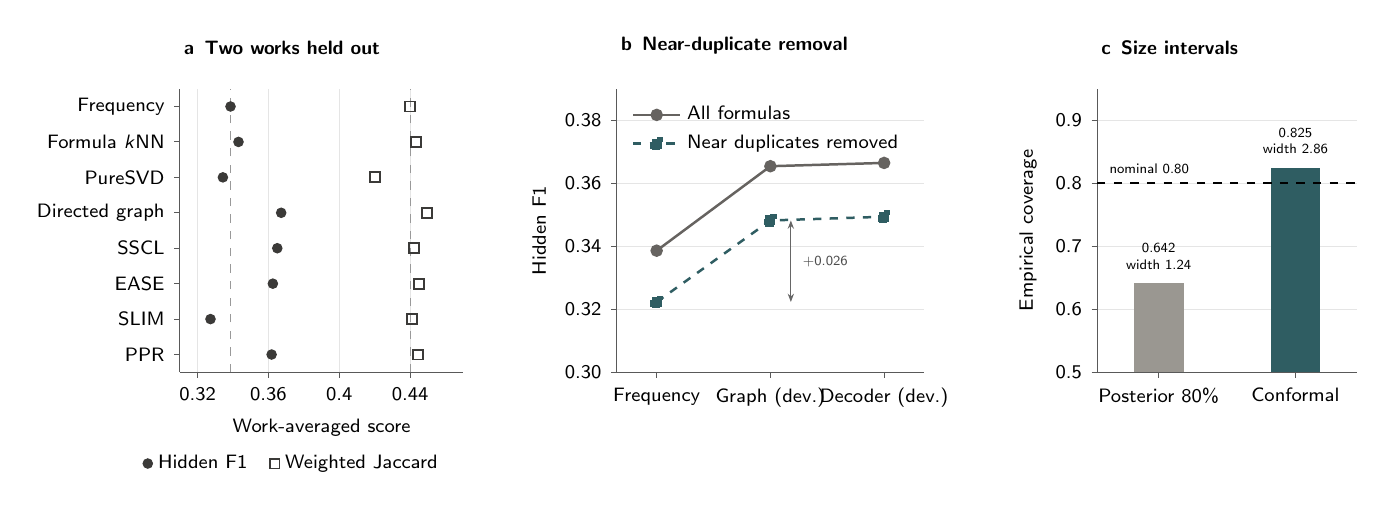
\begin{tikzpicture}
\begin{axis}[paper, at={(1.85cm,0)}, scale only axis, width=3.6cm, height=3.6cm,
  xmin=0.31, xmax=0.47, ymin=0.5, ymax=8.5, ytick={1,...,8},
  yticklabels={PPR,SLIM,EASE,SSCL,Directed graph,PureSVD,Formula $k$NN,Frequency},
  xtick={0.32,0.36,0.40,0.44}, xticklabel style={/pgf/number format/fixed,/pgf/number format/precision=2},
  xlabel={Work-averaged score}, xmajorgrids, title={\textbf{a}\enspace\textbf{Two works held out}},
  legend style={at={(0.4,-0.25)},anchor=north,legend columns=2,/tikz/every even column/.append style={column sep=6pt}}]
\draw[black!40,dashed] (axis cs:0.3386,0.5)--(axis cs:0.3386,8.5) (axis cs:0.4400,0.5)--(axis cs:0.4400,8.5);
\addplot[only marks,mark=*,mark size=1.7pt,color=cdark] coordinates {(0.3386,8) (0.3431,7) (0.3343,6) (0.3672,5) (0.3650,4) (0.3625,3) (0.3273,2) (0.3618,1)};
\addplot[only marks,mark=square,mark size=1.8pt,draw=cdark,line width=0.7pt] coordinates {(0.4400,8) (0.4435,7) (0.4200,6) (0.4494,5) (0.4423,4) (0.4450,3) (0.4408,2) (0.4445,1)};
\legend{Hidden F1,Weighted Jaccard}
\end{axis}
\begin{axis}[paper, at={(7.4cm,0)}, scale only axis, width=3.9cm, height=3.6cm,
  xmin=-0.35, xmax=2.35, ymin=0.30, ymax=0.39, xtick={0,1,2},
  xticklabels={Frequency,Graph (dev.),Decoder (dev.)}, ytick={0.30,0.32,0.34,0.36,0.38},
  yticklabel style={/pgf/number format/fixed,/pgf/number format/precision=2,/pgf/number format/fixed zerofill},
  ylabel={Hidden F1}, ymajorgrids, title={\textbf{b}\enspace\textbf{Near-duplicate removal}},
  legend style={at={(0.02,0.98)},anchor=north west,cells={anchor=west}}]
\addplot[color=cgray,mark=*,mark size=1.8pt,line width=0.9pt] coordinates {(0,0.3386) (1,0.3654197598) (2,0.3664678699)};
\addplot[color=cteal,mark=square*,mark size=1.8pt,line width=0.9pt,dashed] coordinates {(0,0.3223) (1,0.3481871861) (2,0.3493799086)};
\legend{All formulas,Near duplicates removed}
\draw[{Stealth[length=3pt]}-{Stealth[length=3pt]},black!60] (axis cs:1.18,0.3223)--(axis cs:1.18,0.3482);
\node[font=\sffamily\sansmath\tiny,text=black!70,anchor=west] at (axis cs:1.2,0.3352) {$+0.026$};
\end{axis}
\begin{axis}[paper, at={(13.5cm,0)}, scale only axis, width=3.3cm, height=3.6cm,
  ybar, bar width=18pt, ymin=0.5, ymax=0.95, symbolic x coords={Posterior,Conformal}, xtick={Posterior,Conformal}, enlarge x limits=0.45,
  xticklabels={Posterior 80\%,Conformal},
  ytick={0.5,0.6,0.7,0.8,0.9}, yticklabel style={/pgf/number format/fixed,/pgf/number format/precision=1,/pgf/number format/fixed zerofill},
  ylabel={Empirical coverage}, ymajorgrids, title={\textbf{c}\enspace\textbf{Size intervals}}]
\addplot[fill=clgray,draw=none,bar shift=0pt] coordinates {(Posterior,0.642)};
\addplot[fill=cteal,draw=none,bar shift=0pt] coordinates {(Conformal,0.825)};
\draw[black,dashed,line width=0.6pt] (rel axis cs:0,0.6667)--(rel axis cs:1,0.6667);
\node[font=\sffamily\sansmath\tiny,anchor=south west] at (rel axis cs:0.01,0.6667) {nominal 0.80};
\node[font=\sffamily\sansmath\tiny,align=center,anchor=south] at (axis cs:Posterior,0.648) {0.642\\width 1.24};
\node[font=\sffamily\sansmath\tiny,align=center,anchor=south] at (axis cs:Conformal,0.831) {0.825\\width 2.86};
\end{axis}
\end{tikzpicture}
\end{document}
